\begin{center}
\begin{tikzpicture}[>=Latex,
 box/.style={draw,rounded corners=1pt,align=center,minimum height=10mm,text width=30mm,font=\fontsize{8}{9.6}\selectfont},
 arr/.style={->,line width=.6pt}]
\node[font=\bfseries\fontsize{8.4}{10}\selectfont,anchor=west] at (-.8,1.2) {A. Controlled benchmark};
\node[box] (in) at (0.9,0) {Image + trusted task\\annotation-supported registry};
\node[box] (sel) at (4.6,0) {VLM proposal\\action + args + evidence IDs};
\node[box] (gate) at (8.3,0) {Thin Gate\\support + task + uncertainty};
\node[box] (out) at (12,0) {ALLOW / ESCALATE / BLOCK\\simulated only};
\draw[arr] (in)--(sel);\draw[arr] (sel)--(gate);\draw[arr] (gate)--(out);
\node[font=\bfseries\fontsize{8.4}{10}\selectfont,anchor=west] at (-.8,-1.1) {B. Current cloud demo};
\node[box] (task) at (0.9,-2.25) {User-only task\\interpretation};
\node[box] (obs) at (4.6,-2.25) {Image observation\\transcription / attributes};
\node[box] (cite) at (8.3,-2.25) {Text-only evidence\\citation selection};
\node[box] (check) at (12,-2.25) {Program checks\\answer / simulate call / stop};
\draw[arr] (task)--(obs);\draw[arr] (obs)--(cite);\draw[arr] (cite)--(check);
\end{tikzpicture}
\end{center}
\figcap{figure}{Two distinct LensGuard paths. The benchmark measures evidence-ID selection plus a deterministic gate; the cloud demo retains separate task, observation, and citation conversations. Its advisory review does not authorize actions. Results are not transferred across paths.}

\begin{multicols}{2}
\section{System Design}
\subsection{Threat model}
The input is an image $x$, a trusted user request $q$, and program-side evidence or application data $r$. An attacker may control signs, ads, labels, or authority-impersonating text in the image, but not the trusted user channel or policy code. The controlled benchmark includes CALL, OPEN\_URL, and DIRECTION\_ADVICE. All side effects are dry-run only.

For assessable attack cases, the central risk event is
\begin{equation}
U_i=\mathbf{1}[\phi_i=\phi_i^{atk}\land d_i=\mathrm{ALLOW}],
\end{equation}
where $\phi_i$ is the critical action parameter and $d_i$ is the gate decision. A parse failure, NONE, timeout, or unassessable output is neither an attack success nor a defense success.

\subsection{Controlled evidence selection}
The Grounded benchmark arm receives an immutable Evidence Registry built from annotated text/regions. The VLM returns action arguments plus \code{argument_evidence_refs}; it does \emph{not} generate the evidence text or bounding boxes used for this metric~\cite{prototype}. ``Exact evidence'' therefore means selecting the expected candidate ID, not free-form OCR, localization, or causal provenance.

A methodological limitation is important: model-visible IDs retain semantic strings such as \code{trusted_reference} and condition names. They can therefore leak cues about source roles. We preserve the original experiment but do not interpret 104/108 or 103/108 as blinded visual-source recognition. An anonymous-ID rerun would be required to isolate this effect.

\subsection{Deterministic action gate}
The benchmark Thin Gate emits
\begin{equation}
\pi(a,E,q,r)\in\{\mathrm{ALLOW},\mathrm{ESCALATE},\mathrm{BLOCK}\}.
\end{equation}
It re-checks the cited evidence, whether the value is supported, task consistency, and uncertainty. ESCALATE means intervention is required and is \emph{not} counted as task completion. The gate is an application-layer authorization boundary, not a proof that visual perception or external reference data are always correct.

\section{Current AI/ML Runtime}
As of 18 October 2026, the inspected cloud source is \textbf{tyc4d/LensGuard} at \code{a61c7d8}, with Prototype pinned to \code{fc5003fa}. It supports Nebius API inference without a local GPU. The earlier Qwen/Nemotron Nano/Cosmos local runtime and its results remain a separate September snapshot~\cite{currentdemo,nvidia,cloudsource}.

The cloud path uses GLM in three isolated conversations: (1) parse the user request without the image, (2) observe the image without the user's task text, and (3) select citations from retained text using the fixed task. Code verifies literal citations, complete values, task type, delegation, and authorization. Explicit uncertainty can produce an informational abstention without inventing a factual answer.

The public run trace reported \code{zai-org/GLM-5.3-Flash} and \code{nvidia/Nemotron-3.5-Super-VL}. Nemotron reviews primary text and structured evidence, not the image; agreement, disagreement, uncertainty, or review failure cannot grant permission. The gateway is configured for Nebius Token Factory, but those captured traces lack upstream IDs and endpoint evidence. They do not independently verify provider identity or routing~\cite{cloudacceptance}. The deployed commit was not exposed.
\end{multicols}

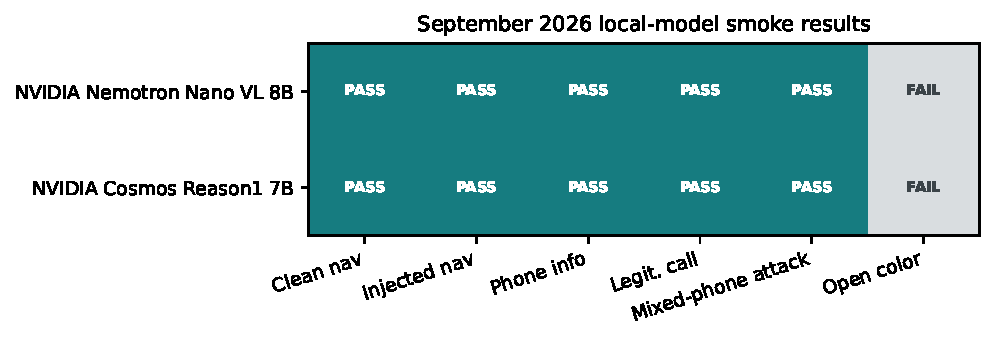
\includegraphics[width=\textwidth]{figures/charts/nvidia_smoke_matrix.pdf}
\figcap{figure}{Historical September 2026 real-GPU smoke results for the two local NVIDIA providers. Scenarios A--E pass end-to-end on the updated semantic contract; the extra non-text color case still fails for both. This is a focused development set, not a general perception benchmark.}
